%!TEX root = ../diploma.tex

\section{Предложенный метод}\label{sec:method}

Предлагается для начала рассмотреть нижеизложенный способ, позволяющий
объединить эвристический метод оптимизации для задачи памяти, изложенный в
работе~\cite{pisarchyk2020efficient}, с описанным в
подразделе~\ref{subsec:literature:parallel} подходом разбиения АГВ на слои
независимых вершин для сокращения затрат на синхронизацию (в частности,
параллельное вычисление вершин).

Введем предикат $F: T\times T \rightarrow \{0,1\}$:
$$F(t_1, t_2) =
\begin{cases}
1, &\text{найдется слой, одновременно использующий $t_1$ и $t_2$}\\
0, &\text{иначе} \end{cases}$$ Использовав его, как дополнительное ограничение
при проверке пересечения времен жизни тензоров, можно сформулировать приведенный
алгоритм~\ref{alg:euristic_search}. Для выполнения алгоритма требуется
предварительно найти времена жизни для всех тензоров, за это отвечает
алгоритм~\ref{alg:lifespans}.

При введении дополнительных ограничений может оказаться, что объем потребляемой
памяти возрастает по сравнению с изначальным алгоритмом. Помимо этого имеется
фактор среднего времени доступа в память ГП (чтение/запись), на который может
влиять кэширование блоков памяти.

С целью варьирования дополнительных ограничений на тензоры, которые не могут
использовать общую память, и количества точек синхронизации, предлагается
дополнительно разбивать каждый слой АГВ на несколько непересекающихся
\textit{групп} одинакового размера (кроме, возможно, последней). Тогда
вычисление отдельно взятого слоя будет представлять собой последовательное
вычисление нескольких групп, между которыми будут установлены дополнительные
точки синхронизации. Новые ограничения на совместное использование памяти
тензорами зададим следующим образом:
\begin{gather*}
    F(t_1, t_2) = \begin{cases}
    1, &\text{найдется группа, одновременно использующая $t_1$ и $t_2$}\\
    0, &\text{иначе} \end{cases}
\end{gather*}

Таким же образом полученный предикат $F(\cdot, \cdot)$ можно использовать в
алгоритме~\ref{alg:euristic_search}.

\begin{figure}
    \centering
    \begin{subfigure}[t]{\textwidth}\centering
    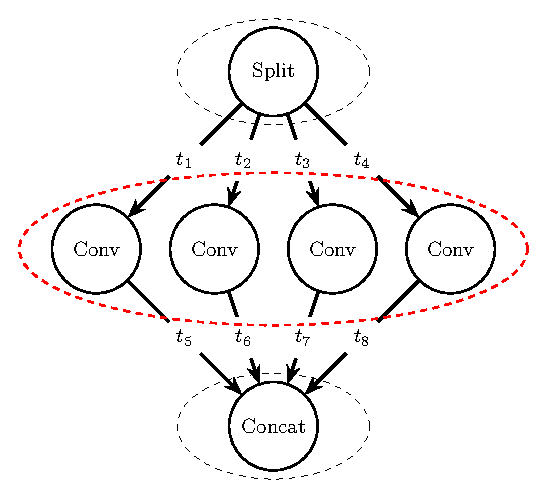
\includegraphics[width=0.6\textwidth]{nogroups}
    \caption{}
    \end{subfigure}
    \begin{subfigure}[t]{\textwidth}\centering
    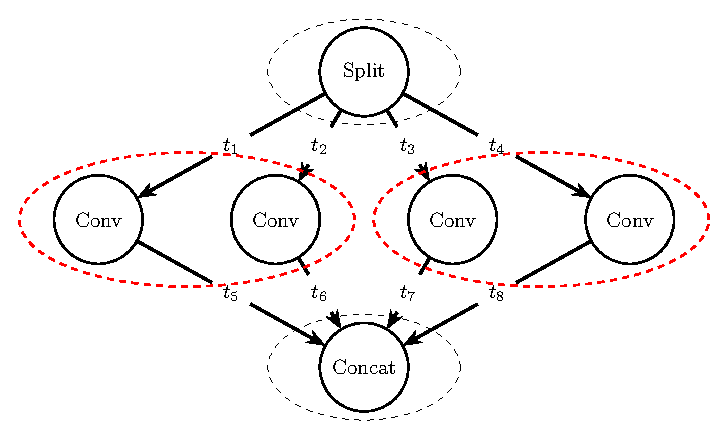
\includegraphics[width=0.8\textwidth]{groups}    
    \caption{}
    \end{subfigure}
    \caption{Пример применения предложенного метода с разбиением на одну группу (а) две группы (б)}
\end{figure}

\begin{algorithm}
    \caption{Нахождение времен жизни тензоров}
    \label{alg:lifespans}
    \begin{algorithmic}[1] % The number tells where the line numbering should start
        \Function{CalculateTensorLifespans}{}
            \State from $\gets\emptyset$ \Comment{ассоциативный массив (тензор, начало времени жизни)}
            \State to $\gets\emptyset$ \Comment{ассоциативный массив (тензор, конец времени жизни)}
            \ForAll{$v_i \in V$ (\textbf{в порядке топологической сортировки})}
                \ForAll{$t$ — входящий/исходящий тензор для $v_i$}
                    \If{$t \notin$ from}
                        \State from($t$) $\gets$ i
                    \EndIf
                    \State to($t$) $\gets$ i
                \EndFor
            \EndFor
            \State lifespan $\gets \left\{[\text{from}(t), \text{to}(t)] \mid t \in T\right\}$
            \State \Return lifespan
        \EndFunction
    \end{algorithmic}
\end{algorithm}

\begin{algorithm}
    \caption{Эвристический поиск распределения памяти}
    \label{alg:euristic_search}
    \begin{algorithmic}[1]
        \Function{CalculateTensorOffsets}{}
            \State lifespan $\gets$ CalculateTensorLifespans()
            \State offset\_records $\gets \emptyset$ \Comment{множество пар (тензор, его сдвиг в памяти)}
            \ForAll{$t$ — промежуточный тензор (\textbf{по убыванию} size($t$))}
                \State prev\_offset $\gets$ 0
                \State best\_offset $\gets$ null
                \State smallest\_gap $\gets \infty$
                \LineComment{пытаемся найти наименьший зазор для $t$}
                \ForAll{(x, offset) $\in$ offset\_records \textbf{по возрастанию} offset}
                    \If{lifespan($t$) $\cap$ lifespan($x$) $\neq \emptyset$ \textbf{или} $F(t, x)=1$}
                        \If{offset $\ge$ prev\_offset}
                            \State gap $\gets$ offset $-$ prev\_offset
                            \If{size$(t)$ $\le$ gap \textbf{и} gap $<$ smallest\_gap}
                                \State smallest\_gap $\gets$ gap
                                \State best\_offset $\gets$ prev\_offset
                            \EndIf
                        \EndIf
                        \State prev\_offset $\gets$ max(prev\_offset, offset + size$(x)$)
                    \EndIf
                \EndFor
                \LineComment{если не нашли зазор, расширяем область памяти}
                \If{best\_offset $=$ null}
                    \State best\_offset $\gets$ prev\_offset
                \EndIf
                \State \textbf{добавляем} (t, best\_offset) \textbf{в} offset\_records
            \EndFor
            \State \Return offset\_records
        \EndFunction
    \end{algorithmic}
\end{algorithm}
\newpage
\noindent\textbf{Планирование запуска АГВ}

При теоретической оценке времени вычисления АГВ будем учитывать следующие
факторы затрат:
\begin{enumerate}
    \item Вычисление вершин/групп вершин
    \item Синхронизации между вычислениями вершин/групп вершин
\end{enumerate}

Время, затраченное на пересылку данных из оперативной памяти в память ГП и
обратно, а также подготовку АГВ к вычислению, учитывать не будем.

Пусть в графе $G=(V,E)$ вершины занумерованы в порядке какой-то топологической
сортировки. Введем обозначения: $\tau(v), v\in V$ — время вычисления вершины
$v$, $s(v_{i}, v_{i+1}), v_{i},v_{i+1}\in V$ — время, затраченное на
синхронизацию между вершинами $v_{i}$ и $v_{i+1}$.

В нашей модели вычислений суммарное затраченное время на вычисление графа $G$
при базовой программной реализации:
$$
\tau(G) = \sum\limits_{i=1}^{n}{\tau(v_i)} + \sum\limits_{i=1}^{n-1}{s(v_{i},v_{i+1})}
$$ 

Используем теперь построенное ранее разбиение на слои для более эффективного
планирования вычислений. Рассмотрим разбиение на слои
$\left\{L_0,\ldots,L_D\right\}$, и для каждого слоя $\tau(L)$ — время вычисления
$L$, $s(L_i, L_{i+1})$ — время, затраченное на синхронизацию между слоями $L_i$
и $L_{i+1}$. Тогда суммарное время вычисления графа $G$:

$$
\tau'(G) = \sum\limits_{i=0}^{D}{\tau(L_i)} + \sum\limits_{i=1}^{D-1}{s(L_{i},L_{i+1})}
$$ 
В таком случае, теоретическое ускорение можно выразить так:
\begin{equation}\label{eqn:speedup}
    S(G) = \frac{\tau(G)}{\tau'(G)} = \frac{\sum\limits_{i=1}^{n}{\tau(v_i)} + \sum\limits_{i=1}^{n-1}{s(v_{i},v_{i+1})}}{\sum\limits_{i=0}^{D}{\tau(L_i)} + \sum\limits_{i=1}^{D-1}{s(L_{i},L_{i+1})}}
\end{equation}
Поскольку при группировке вершин число синхронизаций уменьшается, а в силу роста
степени параллелизма при объединении вершин в группы можно предположить, что
$\tau(L_i) \le \sum\limits_{v\in L_i}\tau(v) \Rightarrow S(G) \ge 1$. В
разделе~\ref{sec:exp} будет протестировано соответствие действительности такой
модели.
